%%%%%%%%%%%%%%%%%%%%%%%%%%%%%%%%%%%%%%%%%%%%%%%%%%%%%%%%%%
\frame {\frametitle{What is an RDD}
%%%%%%%%%%%%%%%%%%%%%%%%%%%%%%%%%%%%%%%%%%%%%%%%%%%%%%%%%%
\begin{itemize}
	\item {\bf RDD are partitioned, locality aware, distributed collections}
	\begin{itemize}
		\item RDD are \emph{immutable}
	\end{itemize}

	\vspace{20pt}

	\item {\bf RDD are data structures that:}
	\begin{itemize}
		\item Either point to a direct data source (e.g. HDFS)
		\item Apply some transformations to its parent RDD(s) to generate new data elements
	\end{itemize}

	\vspace{20pt}

	\item {\bf Computations on RDDs}
	\begin{itemize}
	 	\item Represented by \emph{lazily evaluated} lineage \emph{DAGs} composed by chained RDDs
	 \end{itemize} 
\end{itemize}
}

%%%%%%%%%%%%%%%%%%%%%%%%%%%%%%%%%%%%%%%%%%%%%%%%%%%%%%%%%%
\frame {\frametitle{RDD Abstraction}
%%%%%%%%%%%%%%%%%%%%%%%%%%%%%%%%%%%%%%%%%%%%%%%%%%%%%%%%%%
\begin{itemize}
	\item {\bf Overall objective}
	\begin{itemize}
		\item Support a wide array of operators (more than just \texttt{Map} and \texttt{Reduce})
		\item Allow arbitrary composition of such operators
	\end{itemize}

	\vspace{20pt}

	\item {\bf Simplify scheduling}
	\begin{itemize}
		\item Avoid to modify the scheduler for each operator
	\end{itemize}

	\vspace{20pt}

	\item[$\to$] The question is: \emph{How to capture dependencies in a general way?}
\end{itemize}
}

%%%%%%%%%%%%%%%%%%%%%%%%%%%%%%%%%%%%%%%%%%%%%%%%%%%%%%%%%%
\frame {\frametitle{RDD Interfaces}
%%%%%%%%%%%%%%%%%%%%%%%%%%%%%%%%%%%%%%%%%%%%%%%%%%%%%%%%%%
\begin{itemize}
	\item {\bf Set of partitions (``splits'')}
	\begin{itemize}
		\item Much like in Hadoop MapReduce, each RDD is associated to (input) partitions
	\end{itemize}

	\item {\bf List of dependencies on parent RDDs}
	\begin{itemize}
		\item This is completely new w.r.t. Hadoop MapReduce
	\end{itemize}

	\item {\bf Function to compute a partition given parents}
	\begin{itemize}
		\item This is actually the ``user-defined code'' we referred to when discussing about the \texttt{Mapper} and \texttt{Reducer} classes in Hadoop
	\end{itemize}

	\item {\bf Optional preferred locations}
	\begin{itemize}
		\item This is to enforce data locality
	\end{itemize}

	\item {\bf Optional partitioning info (Partitioner)}
	\begin{itemize}
		\item This really helps in some ``advanced'' scenarios in which you want to pay attention to the behavior of the shuffle mechanism
	\end{itemize}
\end{itemize}
}

%%%%%%%%%%%%%%%%%%%%%%%%%%%%%%%%%%%%%%%%%%%%%%%%%%%%%%%%%%
\frame {\frametitle{Hadoop RDD}
%%%%%%%%%%%%%%%%%%%%%%%%%%%%%%%%%%%%%%%%%%%%%%%%%%%%%%%%%%
\begin{itemize}
	\item {\color{mauve} partitions} = one per HDFS block

	\vspace{10pt}

	\item {\color{mauve} dependencies} = none

	\vspace{10pt}

	\item {\color{mauve} compute(partition)} = read corresponding block

	\vspace{10pt}

	\item {\color{mauve} preferredLocations(part)} = HDFS block location

	\vspace{10pt}

	\item {\color{mauve} partitioner} = none

\end{itemize}
}

%%%%%%%%%%%%%%%%%%%%%%%%%%%%%%%%%%%%%%%%%%%%%%%%%%%%%%%%%%
\frame {\frametitle{Filtered RDD}
%%%%%%%%%%%%%%%%%%%%%%%%%%%%%%%%%%%%%%%%%%%%%%%%%%%%%%%%%%
\begin{itemize}
	\item {\color{mauve} partitions} = same as parent RDD

	\vspace{10pt}

	\item {\color{mauve} dependencies} = \emph{one-to-one} on parent

	\vspace{10pt}

	\item {\color{mauve} compute(partition)} = compute parent and filter it

	\vspace{10pt}

	\item {\color{mauve} preferredLocations(part)} = none (\emph{ask parent})

	\vspace{10pt}

	\item {\color{mauve} partitioner} = none

\end{itemize}
}

%%%%%%%%%%%%%%%%%%%%%%%%%%%%%%%%%%%%%%%%%%%%%%%%%%%%%%%%%%
\frame {\frametitle{Joined RDD}
%%%%%%%%%%%%%%%%%%%%%%%%%%%%%%%%%%%%%%%%%%%%%%%%%%%%%%%%%%
\begin{itemize}
	\item {\color{mauve} partitions} = one per reduce task

	\vspace{10pt}

	\item {\color{mauve} dependencies} = \emph{shuffle} on \emph{each} parent

	\vspace{10pt}

	\item {\color{mauve} compute(partition)} = read and join shuffled data

	\vspace{10pt}

	\item {\color{mauve} preferredLocations(part)} = none 

	\vspace{10pt}

	\item {\color{mauve} partitioner} = HashPartitioner(numTask)\footnote{Spark knows this data is hashed.}

\end{itemize}
}

%%%%%%%%%%%%%%%%%%%%%%%%%%%%%%%%%%%%%%%%%%%%%%%%%%%%%%%%%%
\frame {\frametitle{Dependency Types}
%%%%%%%%%%%%%%%%%%%%%%%%%%%%%%%%%%%%%%%%%%%%%%%%%%%%%%%%%%
\begin{columns}[t, onlytextwidth]
	\begin{column}[T]{.4\textwidth}
		\begin{center}
			{ \tiny \bf Narrow dependencies}
		\end{center}
		\begin{figure}[h]
			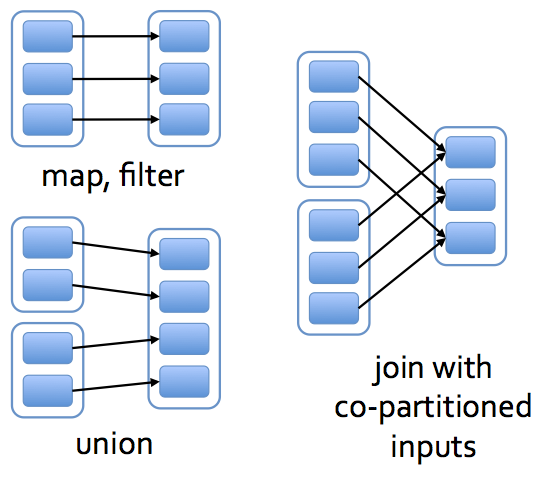
\includegraphics[scale=0.3]{./Figures/narrow_deps}
		\end{figure}
	\end{column}

	\begin{column}[T]{.4\textwidth}
		\begin{center}
			{ \tiny \bf Wide dependencies}
		\end{center}
		\begin{figure}[h]
			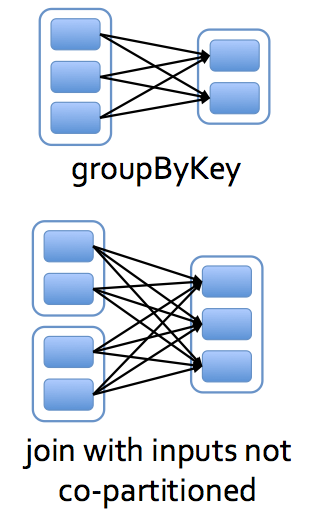
\includegraphics[scale=0.3]{./Figures/wide_deps}
		\end{figure}
	\end{column}
\end{columns}
}

%%%%%%%%%%%%%%%%%%%%%%%%%%%%%%%%%%%%%%%%%%%%%%%%%%%%%%%%%%
\frame {\frametitle{RDD Code Snippet}
%%%%%%%%%%%%%%%%%%%%%%%%%%%%%%%%%%%%%%%%%%%%%%%%%%%%%%%%%%
	\begin{figure}[h]
	\center
		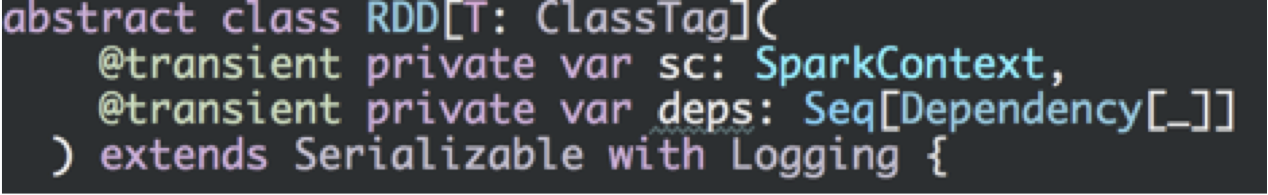
\includegraphics[scale=0.5]{./Figures/rdd_snippet}
	\end{figure}


	\begin{itemize}
		\item {\bf SparkContext}
		\begin{itemize}
			\item This is the main entity responsible for setting up a job
			\item Contains SparkConfig, Scheduler, entry point of running jobs (runJobs)
		\end{itemize}

		\vspace{15pt}

		\item {\bf Dependencies}
		\begin{itemize}
			\item Input RDD(s)
		\end{itemize}
	\end{itemize}

	\begin{colorblock}{blue}{lightblue}{}
	{\bf M. Zaharia}, M. Chowdhury, T. Das, A. Dave, J. Ma, M. McCauley, M.J. Franklin, S. Shenker, I. Stoica. \emph{Resilient Distributed Datasets: A Fault-Tolerant Abstraction for In-Memory Cluster Computing}, {\bf NSDI}, 2012		
	\end{colorblock}			
}

%%%%%%%%%%%%%%%%%%%%%%%%%%%%%%%%%%%%%%%%%%%%%%%%%%%%%%%%%%
\frame {\frametitle{RDD.map operation Snippet}
%%%%%%%%%%%%%%%%%%%%%%%%%%%%%%%%%%%%%%%%%%%%%%%%%%%%%%%%%%
	\begin{itemize}
		\item {\bf Map: RDD[T] $\to$ RDD[U]}
	\end{itemize}

	\begin{figure}[h]
	\center
		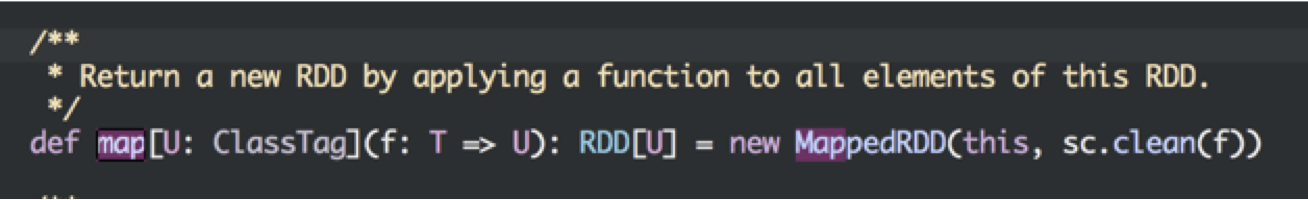
\includegraphics[scale=0.5]{./Figures/rddmap_snippet}
	\end{figure}

	\begin{itemize}
		\item {\bf MappedRDD}
		\begin{itemize}
			\item For each element in a partition, apply function $f$
		\end{itemize}
	\end{itemize}

	\begin{figure}[h]
	\center
		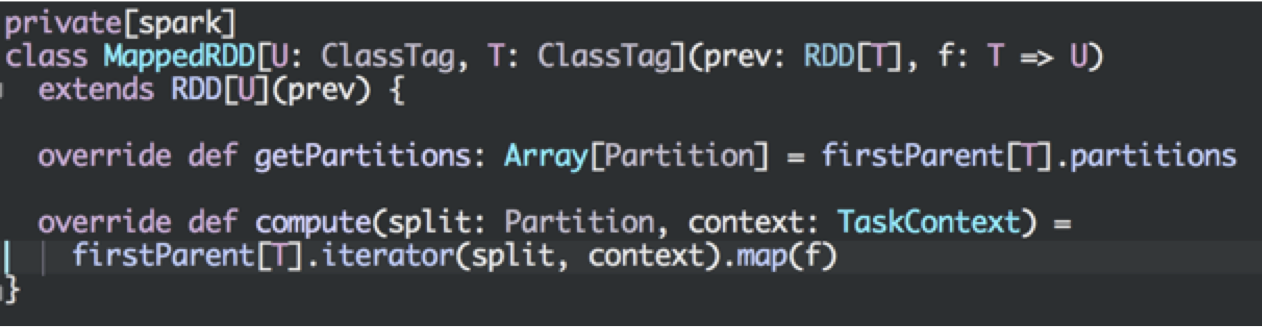
\includegraphics[scale=0.5]{./Figures/mappedrdd_snippet}
	\end{figure}

}

%%%%%%%%%%%%%%%%%%%%%%%%%%%%%%%%%%%%%%%%%%%%%%%%%%%%%%%%%%
\frame {\frametitle{RDD Iterator Code Snipped}
%%%%%%%%%%%%%%%%%%%%%%%%%%%%%%%%%%%%%%%%%%%%%%%%%%%%%%%%%%
\begin{itemize}
	\item {\bf Method to go through an RDD and apply function $f$}
	\begin{itemize}
		\item First, check local cache
		\item If not found, compute the RDD
	\end{itemize}
\end{itemize}

	\begin{figure}[h]
	\center
		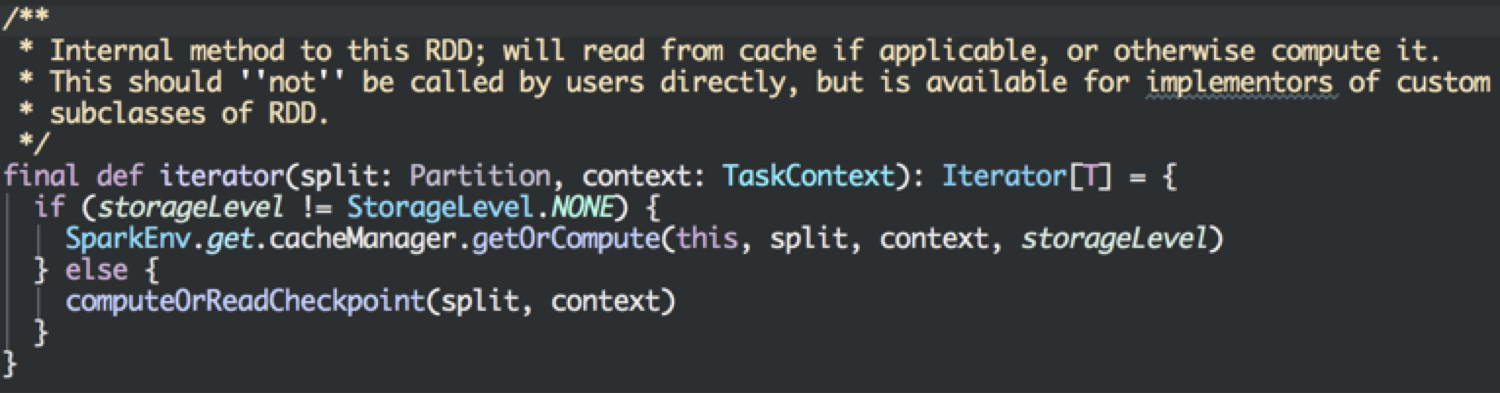
\includegraphics[scale=0.45]{./Figures/iterator_snippet}
	\end{figure}


\begin{itemize}
	\item {\bf Storage Levels}
	\begin{itemize}
		\item Disk
		\item Memory
		\item Off Heap (e.g. external memory stores like Tachyon)
		\item De-serialized
	\end{itemize}
\end{itemize}

}

%%%%%%%%%%%%%%%%%%%%%%%%%%%%%%%%%%%%%%%%%%%%%%%%%%%%%%%%%%
\frame {\frametitle{Making RDD from local collections}
%%%%%%%%%%%%%%%%%%%%%%%%%%%%%%%%%%%%%%%%%%%%%%%%%%%%%%%%%%
	\begin{itemize}
		\item {\bf Convert a local (on the driver) Seq[T] into RDD[T]}
	\end{itemize}

	\begin{figure}[h]
	\center
		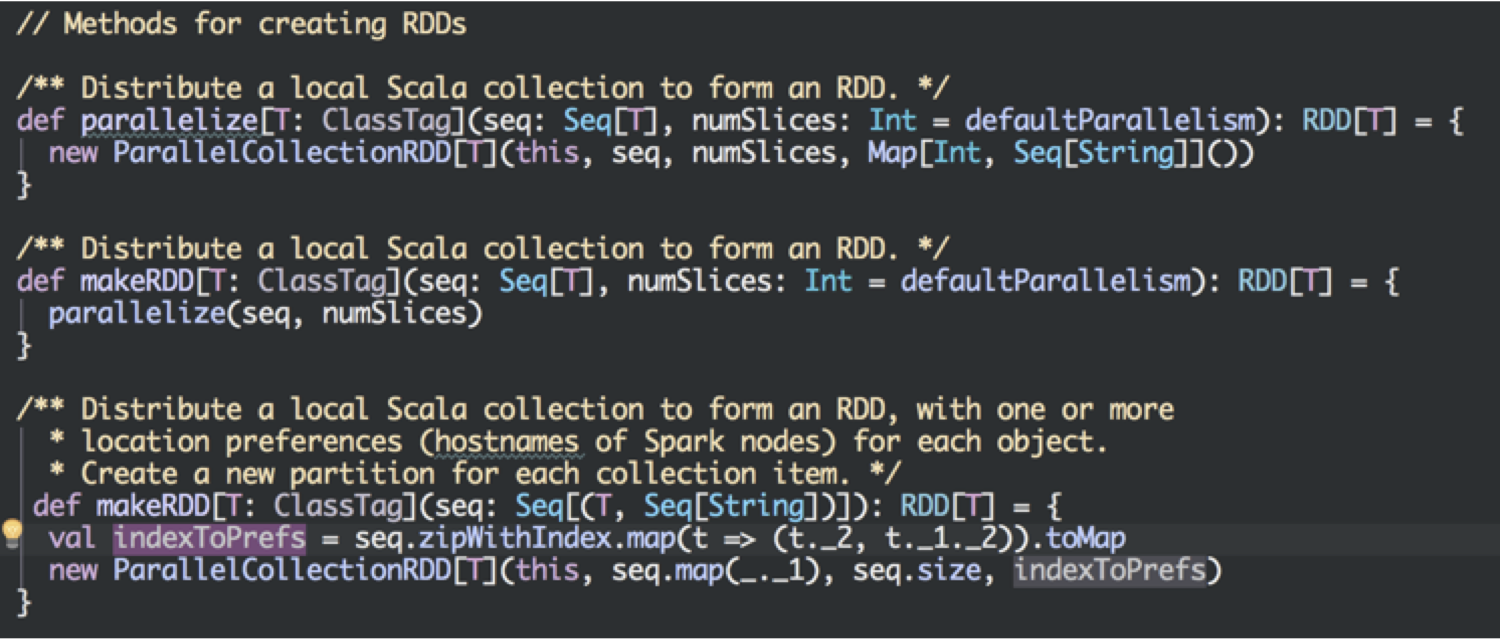
\includegraphics[scale=0.45]{./Figures/parallelize_snippet}
	\end{figure}


}

%%%%%%%%%%%%%%%%%%%%%%%%%%%%%%%%%%%%%%%%%%%%%%%%%%%%%%%%%%
\frame {\frametitle{Hadoop RDD Code Snippet}
%%%%%%%%%%%%%%%%%%%%%%%%%%%%%%%%%%%%%%%%%%%%%%%%%%%%%%%%%%
\begin{itemize}
	\item {\bf Reading HDFS data as <key, value> records}
\end{itemize}

\begin{figure}[h]
	\center
		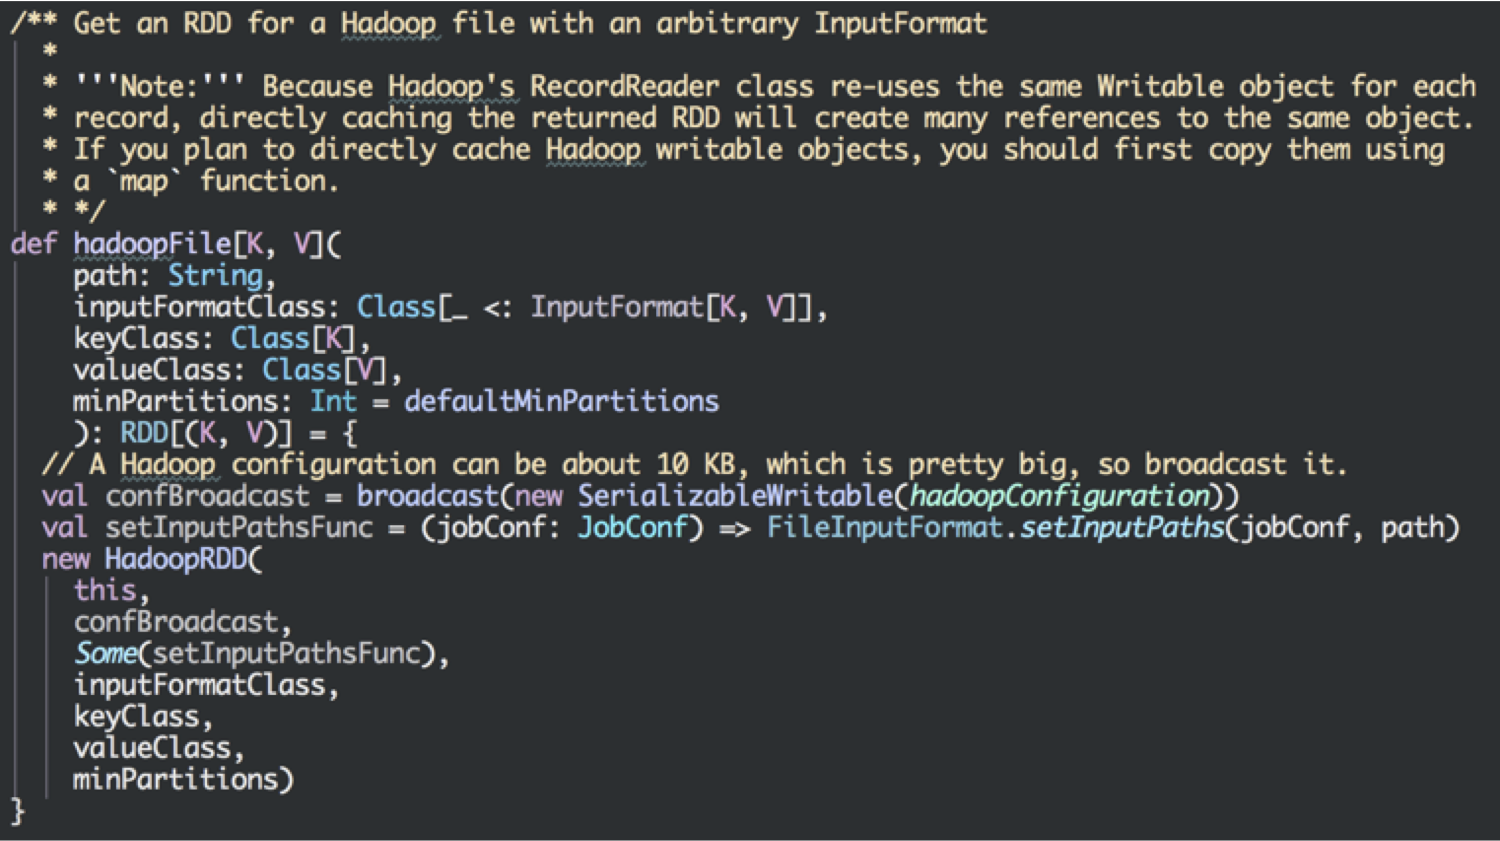
\includegraphics[scale=0.45]{./Figures/HadoopRDD_snippet}
\end{figure}
}
